\documentclass[class=report, crop=false, 12pt,a4paper]{standalone}
\usepackage{enumitem}
\usepackage{multicol}
\usepackage{graphicx}
\usepackage{float}
\usepackage{amsmath}
\usepackage{amssymb}
\usepackage{mathtools}
\usepackage{siunitx}
\usepackage{commath}
\usepackage{array}
\usepackage{natbib}
\usepackage{caption}
\usepackage{subcaption}
\usepackage[a4paper,width=150mm,top=25mm,bottom=25mm]{geometry}
\setlength{\parindent}{0pt}
\begin{document}
\section{Introduction}
\subsection{What is the module about?}
\begin{quotation}
    Dynamics: the study of forces and the resultant motion.
\end{quotation}
In this module we will study the oscillatory forces and the resulted motion of bodies, in other words "Mechanical Vibration."
\begin{itemize}
    \item Harmful vibrations:
    \begin{itemize}
        \item Vibrations can cause:
        \begin{itemize}
            \item Resonance
            \item Flutter
            \item Fatigue
        \end{itemize}
        \item It may cause discomfort and even be harmful to the human.
    \end{itemize}
    \item Good vibrations:
    \begin{itemize}
        \item Hearing
        \item Loudspeakers
        \item Musical instruments
        \item Electric toothbrush
        \item Clocks
        \item Material handling
        \item Sifting
    \end{itemize}
\end{itemize}
\subsection{How to deal?}
Analysis:
\begin{itemize}
    \item Mathematical modelling
    \item Derivation of governing equations
    \item Solution of the governing equations
    \item Interpretation of results
\end{itemize}
Measurements:
\begin{itemize}
    \item Appropriate setup
    \item Interpretation of measurements
    \item Updating mathematical models
\end{itemize}
\subsection*{How would this module enable you to analyse dynamical systems?}
\begin{itemize}
    \item Mathematical modelling, week 1 also 2-11.
    \item Single degree of freedom systems
    \begin{itemize}
        \item Free vibration
        \begin{itemize}
            \item Undamped, weeks 1 and 2
            \item Damped, week 3
        \end{itemize}
        \item Forced vibration of single degree of freedom system
        \begin{itemize}
            \item Harmonic excitation, weeks 4 and 5
            \item Arbitrary excitation, week 7
        \end{itemize}
    \end{itemize}
    \item Two degree of freedom system, week 8
    \item Multi degree of freedom systems, week 9
    \item The use of computer aided engineering to create a refined motor vehicle, invited talk, week 10
    \item Introduction to continuous systems, week 11
    \item Vibration measurements
    \item Vibration control
\end{itemize}
\section{Fundamentals}
\subsection{Physical elements of vibrations}
\begin{quotation}
    Vibration: A vibration or oscillation is a periodic motion, i.e. it repeats itself in all its particular after a certain interval of time.
\end{quotation}
In general in any mechanical oscillatory system there are:
\begin{itemize}
    \item A \textbf{mass} that can store kinetic energy (accelerates when a load is applied upon)
    \item A \textbf{spring} that can store potential energy (constant displacement due to a constant force)
    \item A \textbf{damper} through which energy dissipates
\end{itemize}
What are the equivalent electrical elements?
\begin{itemize}
    \item Force ($F$) - Voltage ($V$)
    \item Mass ($M$) - Inductance ($L$)
    \item Damping ($B$) - Resistance ($R$)
    \item Spring constant ($K$) - Reciprocal of Capacitance ($\frac{1}{c}$)
    \item Displacement ($x$) - Charge ($q$)
    \item Velocity ($v$) - Current ($i$)
\end{itemize}
In other words vibration is a result of the interaction of two forces. One a function of displacement (spring):
\begin{gather}
    f)k = - kx(t)
\end{gather}
One a function of acceleration (mass):
\begin{gather}
    f_m = m \ddot{x} (t)
\end{gather}
\begin{figure}[H]
    \centering
    \begin{minipage}{.5\textwidth}
      \centering
      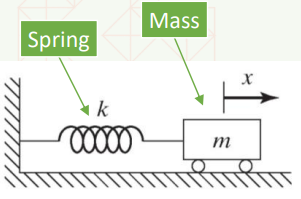
\includegraphics[width=.8\linewidth]{../img/diagram1.jpg}
      \captionof{figure}{Spring-mass system.}
    \end{minipage}%
    \begin{minipage}{.5\textwidth}
      \centering
      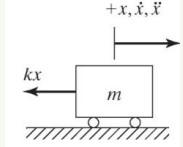
\includegraphics[width=.8\linewidth]{../img/diagram2.jpg}
      \captionof{figure}{free body diagram.}
    \end{minipage}
\end{figure}
Equation of motion:
\begin{align}
    \sum F &= m\ddot{x} (t)\\
    m\ddot{x}(t) &= -kx(t)
\end{align}
Equation of motion:
\begin{gather}
    m\ddot{x}(t) + kx(t) = 0
\end{gather}
Solution:
\begin{gather}
    x(t) = A\sin \left(\omega_n t + \phi \right)
\end{gather}
\subsection{Degree of freedom}
The minimum number of coordinates that are required to define the position of a system is called degree of freedom. 
\begin{itemize}
    \item Single degree of freedom (SDOF):
    \begin{itemize}
        \item Only one coordinate is required to fully define the state of the system
    \end{itemize}
\end{itemize}
\begin{figure}[H]
    \centering
    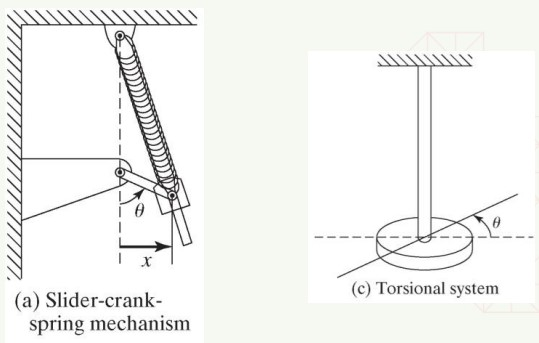
\includegraphics[width = 0.8\textwidth]{../img/diagram3.jpg}
    \caption{SDOF systems.}
\end{figure}
\begin{figure}[H]
    \centering
    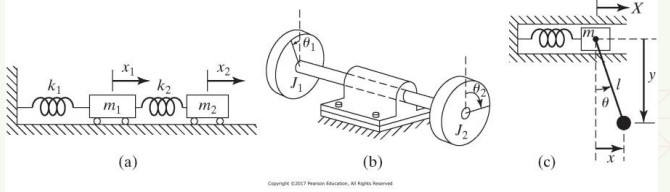
\includegraphics[width = 0.8\textwidth]{../img/diagram4.jpg}
    \caption{Two degree of freedom systems.}
\end{figure}
\begin{figure}[H]
    \centering
    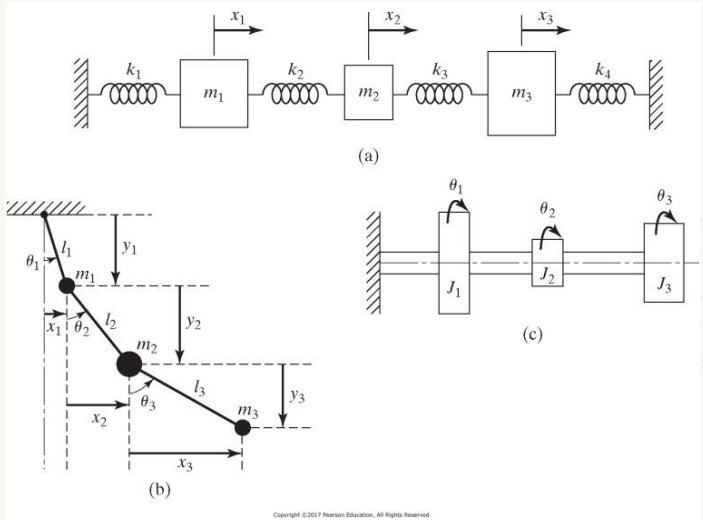
\includegraphics[width = 0.8\textwidth]{../img/diagram5.jpg}
    \caption{Three degree of freedom systems.}
\end{figure}
\subsection{Continuous systems}
Some systems, especially those involving continuous elastic members, have an infinite number of degrees of freedom.
\begin{figure}[H]
    \centering
    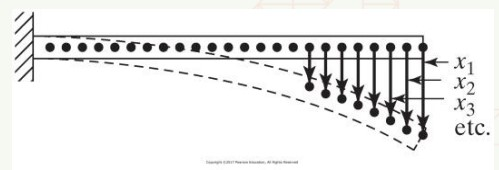
\includegraphics[width = 0.8\textwidth]{../img/diagram6.jpg}
    \caption{Continuous degree of freedom.}
\end{figure}
\textbf{Discrete or lumped parameter systems:} A system with finite number of degree of freedom.
Continuous or distributed systems: an infinite number of degree of freedom.
\subsection{Analysis procedure}
\subsubsection{Mathematical modelling}
We need a mathematical model to obtain a solution for the vibrational problem. The model is a compromise between simplicity and accuracy. We make some assumption and our model is valid with the limitation of those assumptions only. 
\begin{figure}[H]
    \centering
    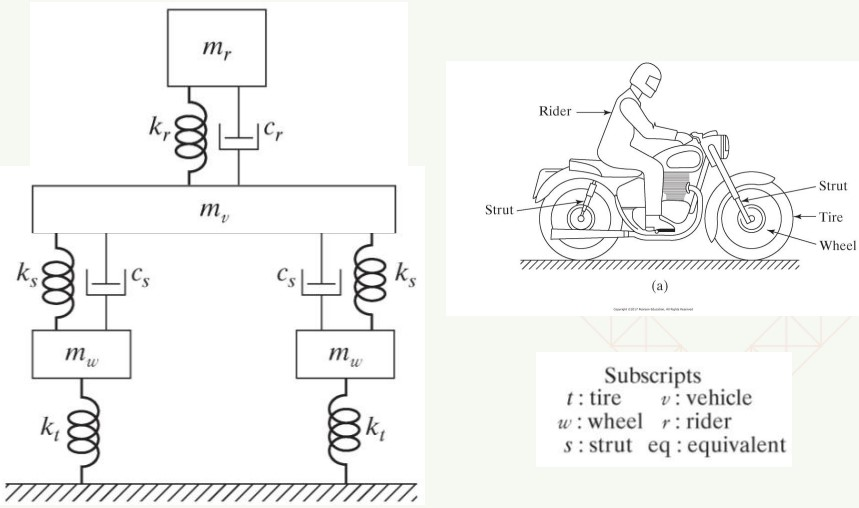
\includegraphics[width = 0.8\textwidth]{../img/diagram7.jpg}
    \caption{Model of rider-motorbike-wheel system.}
\end{figure}
\begin{figure}[H]
    \centering
    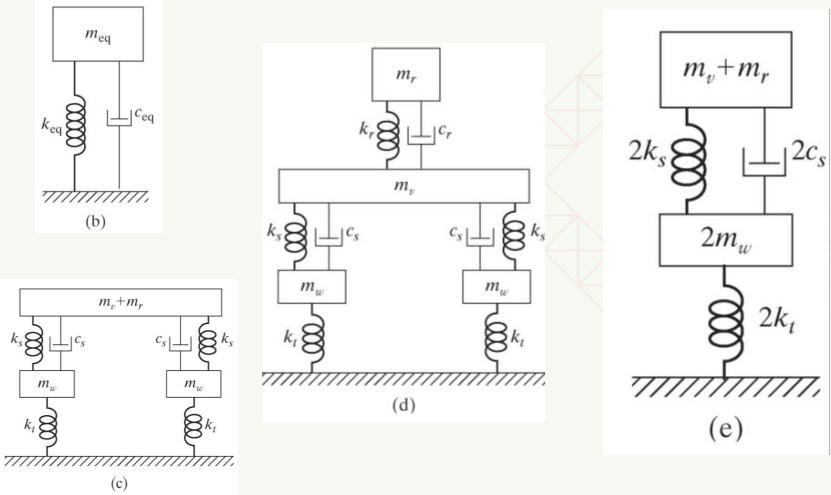
\includegraphics[width = 0.8\textwidth]{../img/diagram8.jpg}
    \caption{Various models of rider-motorbike-wheel system.}
\end{figure}
\begin{figure}[H]
    \centering
    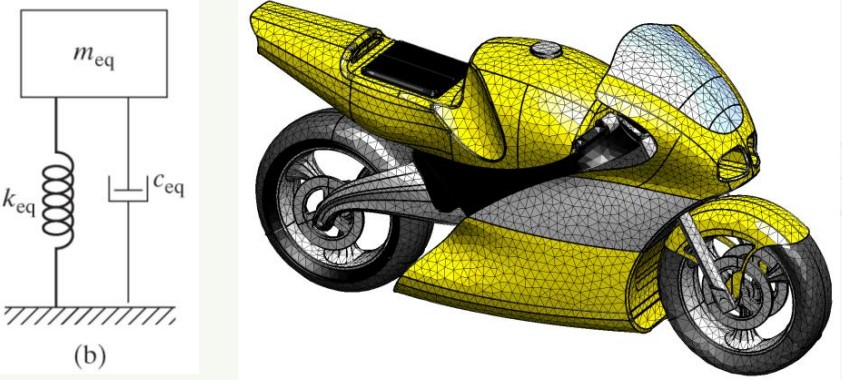
\includegraphics[width = 0.8\textwidth]{../img/diagram9.jpg}
    \caption{Complex model of rider-motorbike-wheel system.}
\end{figure}
\subsubsection{Derivation of governing equations}
Apply principle of dynamics to obtain the equations:
\begin{itemize}
    \item Newton's second law of motion
    \item d'Alembert's principle
    \item The principle of conservation of energy
\end{itemize}
Usually in the form of a set of ordinary differential equations.
\subsubsection{Solution of governing equations}
\begin{itemize}
    \item Standard method of solving differential equations
    \item Laplace transformation method
    \item Matrix methods
    \item Numerical methods
\end{itemize}
\subsubsection{Interpretation of results}
\begin{itemize}
    \item Have a clear view of the purpose of the analysis
    \item Pay attention to the assumption made to obtain the results.
\end{itemize}
\subsection{Classification of vibration}
\begin{figure}[H]
    \centering
    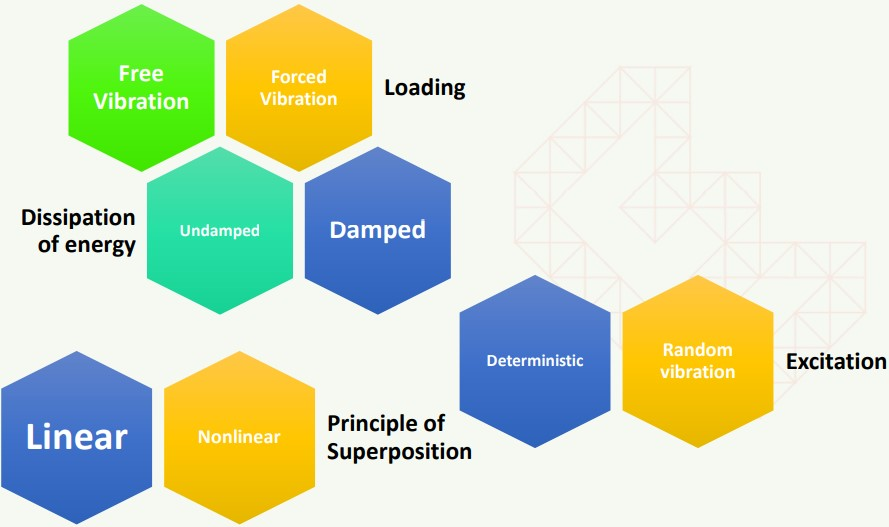
\includegraphics[width = 0.8\textwidth]{../img/diagram10.jpg}
    \caption{Classification of vibrations.}
\end{figure}
\subsection{Example: simple pendulum}
Deriving the equation of motion. We have some assumptions:
\begin{itemize}
    \item The mass of the rod is ignored
    \item Friction in the hinges is ignored
    \item The motion remains in a plane
\end{itemize}
\begin{figure}[H]
    \centering
    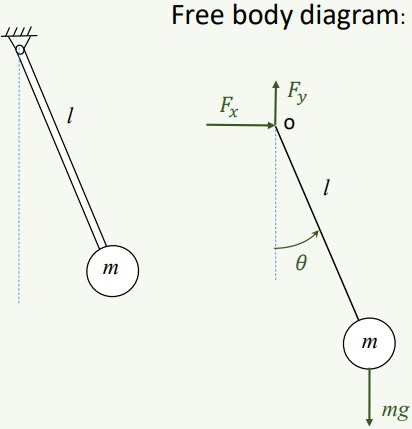
\includegraphics[width = 0.5\textwidth]{../img/diagram11.jpg}
    \caption{Free body diagram of simple pendulum system.}
\end{figure}
Euler's second law:
\begin{align}
    \sum M_o &= J \alpha\\
    J \alpha(t) &= - mgl\sin \theta (t)\\
    ml^2 \ddot{\theta} (t) + mgl\sin \theta (t) &= 0 
\end{align}
Linearisation:
\begin{align}
    \ddot{\theta} (t) + \frac{g}{l}\theta(t) =0
\end{align}
\subsection{Simple harmonic motion}
\begin{figure}[H]
    \centering
    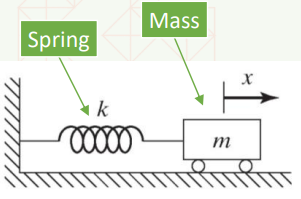
\includegraphics[width = 0.5\textwidth]{../img/diagram1.jpg}
    \caption{Spring-mass system.}
\end{figure}
\begin{align}
    x(t) &= A \sin\left(\omega_n t + \phi\right)\\
    \dot{x} &= A \omega_n \cos \left(\omega_n t + \phi\right)\\
    \ddot{x} &= - A \omega_n^2 \sin \left(\omega_n t + \phi\right)
\end{align}
Substitute in equation of motion:
\begin{gather}
    -m A \omega_n^2 \sin\left(\omega_n t + \phi\right) + k A \sin \left(\omega_n t + \phi \right) = 0\\
    \omega_n^2 = \frac{k}{n} \textrm{ or } \omega_n = \sqrt{\frac{k}{m}} \label{naturalFrequency}
\end{gather}
where \ref{naturalFrequency} is the natural frequency.
\subsection{Amplitude and phase}
\begin{gather}
    x(t) = A \sin\left(\omega_n t + \phi\right)
\end{gather}
Initial conditions: initial displacement $x_0$ and initial velocity $v_0$ of the mass. 
\begin{gather}
    x_0 = x(t = 0) = A\sin \phi\\
    v_0 = \dot{x} (t=0) = A\omega_n \cos\left(\omega_n x_0 + \phi\right) = A \omega_n \cos \phi\\
    \frac{v_0}{\omega_n} = A \cos \phi\\
    x_0^2 + \frac{v_0^2}{\omega_n^2} = A^2 \sin^2 \phi + A^2 \cos^2 \phi = A^2\\
    \frac{\sin \phi}{\cos \phi} = \dfrac{x_0}{\dfrac{v_0}{\omega_n}}
\end{gather}
Thus:
\begin{gather}
    A = \dfrac{\sqrt{\omega_n^2 x_0^2 + v_0^2}}{\omega_n} \textrm{ and } \phi = \arctan{\dfrac{\omega_n x_0}{v_0}}
\end{gather}
\begin{figure}[H]
    \centering
    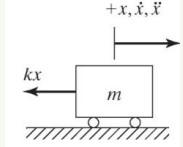
\includegraphics[width = 0.3\textwidth]{../img/diagram2.jpg}
    \caption{Free body diagram of spring-mass system.}
\end{figure}
\begin{gather}
    m = \SI{2}{\kg} \textrm{ and } k = \SI{200}{\newton\per\meter}\\
    1. \; x_0 = \SI{-2}{\milli\meter} \textrm{ and } v_0 = \SI{10}{\milli\meter\per\second}\\
    2. \; x_0 = \SI{2}{\milli\meter} \textrm{ and } v_0 = \SI{-10}{\milli\meter\per\second}
\end{gather}
Solution:
\begin{align}
    \omega_n &= \sqrt{\dfrac{k}{m}} = \sqrt{\dfrac{200}{2}} = \SI{200}{\radian\per\second}\\
    A &= \dfrac{\sqrt{\omega_n^2 x_0^2 + v_0^2}}{\omega_n} = \dfrac{\sqrt{10^2 \cdot 2^2 + 10^2}}{10} = \SI{2.2}{\milli\meter}\\
    1. \; \phi &= \arctan\left(\dfrac{\omega_n x_0}{v_0}\right) = \arctan\left(\dfrac{10\cdot-2}{10}\right) = \SI{-1.107}{\radian} \textrm{ or } \SI{-63.4}{\degree}\\
    2. \; \phi &= \arctan\left(\dfrac{\omega_n x_0}{v_0}\right) = \arctan\left(\dfrac{10\cdot-2}{10}\right) = \left(-1.107+\pi\right)\si{\radian} \textrm{ or } \SI{116.6}{\degree}
\end{align}
\begin{figure}[H]
    \centering
    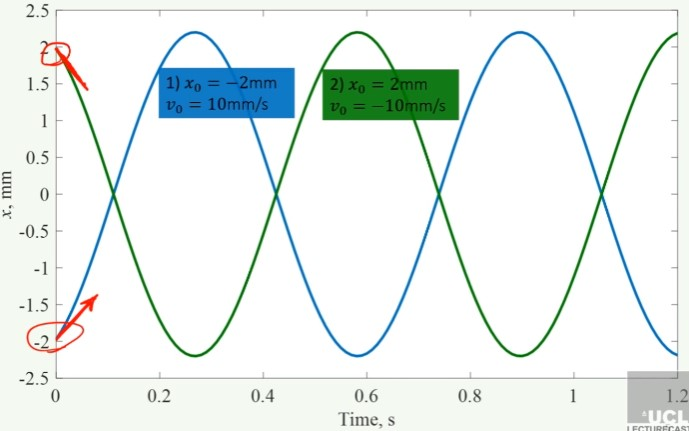
\includegraphics[width = 0.8\textwidth]{../img/diagram12.jpg}
    \caption{Plots of SHM.}
\end{figure}
\begin{figure}[H]
    \centering
    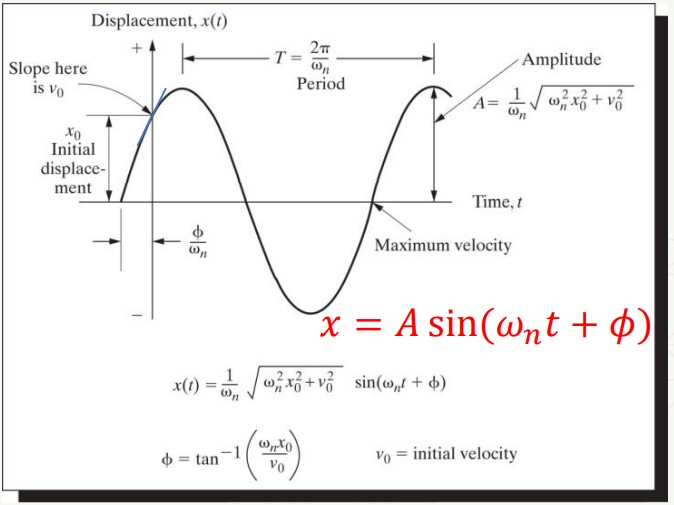
\includegraphics[width = 0.8\textwidth]{../img/diagram13.jpg}
    \caption{Analysis of SHM plots.}
\end{figure}
\subsection{Springs}
Hooke's law (linear spring):
\begin{equation}
    F_k = kx
\end{equation}
\begin{figure}[H]
    \centering
    \begin{minipage}{.5\textwidth}
      \centering
      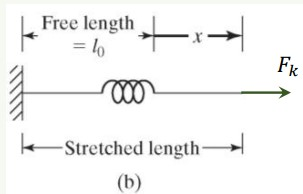
\includegraphics[width=.8\linewidth]{../img/diagram14.jpg}
      \captionof{figure}{Spring system.}
    \end{minipage}%
    \begin{minipage}{.5\textwidth}
      \centering
      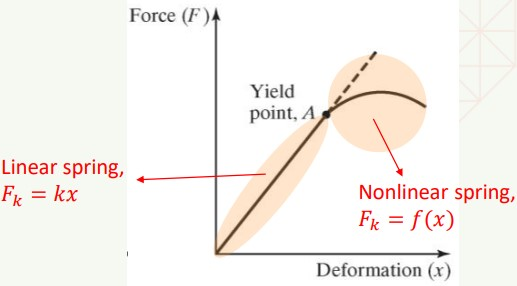
\includegraphics[width=.8\linewidth]{../img/diagram15.jpg}
      \captionof{figure}{$F$ vs $x$ of spring.}
    \end{minipage}
\end{figure}
\subsection{Modelling springs}
Springs in parallel:
\begin{align}
    W &= k_1 \delta_{st} + k_2 \delta_{st}\\
    &= \left(k_1 + k_2 \right)\delta_{st}\\
    W &= k_{eq} \delta_{st}\\
    k_{eq} &= \left(k_1 + k_2\right)
\end{align}
\begin{figure}[H]
    \centering
    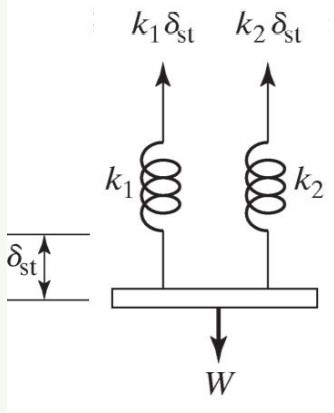
\includegraphics[width = 0.4\textwidth]{../img/diagram16.jpg}
    \caption{Parallel springs.}
\end{figure}
Springs in series:
\begin{align}
    \delta_{st} &= \delta_1 + \delta_2\\
    w &= k_1 \delta_1\\
    w &= k_2 \delta_2
\end{align}
or
\begin{align}
    \delta_{st} &= \dfrac{w}{k_1} + \dfrac{w}{k_2}\\
    \delta_{st} &= \dfrac{w}{k_{eq}}\\
    k_{eq} &= \dfrac{k_1k_2}{k_1 + k_2}
\end{align}
\begin{figure}
    \centering
    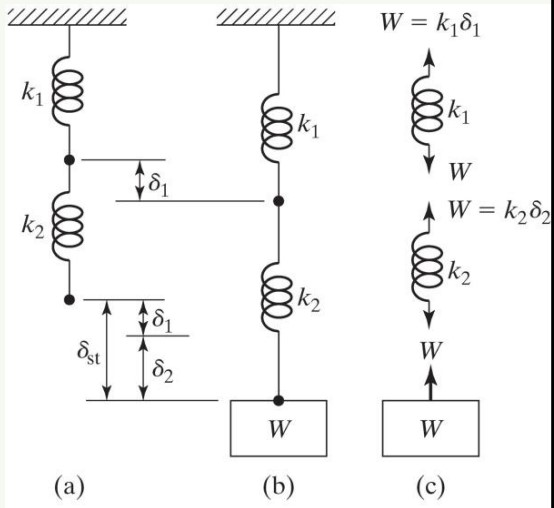
\includegraphics[width = 0.4\textwidth]{../img/diagram17.jpg}
    \caption{Series springs.}
\end{figure}
A cantilever beam with a mass at the free end:
\begin{align}
    \delta_{st} &= \dfrac{Wl^3}{3EI}\\
    k_{eq} &= \dfrac{W}{\delta_{st}}\\
    k_{eq} &= \dfrac{3EI}{l^3}
\end{align}
\begin{figure}[H]
    \centering
    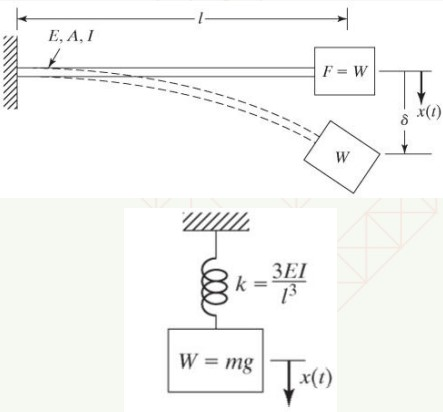
\includegraphics[width = 0.6\textwidth]{../img/diagram18.jpg}
    \caption{Cantilever beam with mass at free end.}
\end{figure}
\subsection{Longitudinal motion of a bar}
\begin{figure}[H]
    \centering
    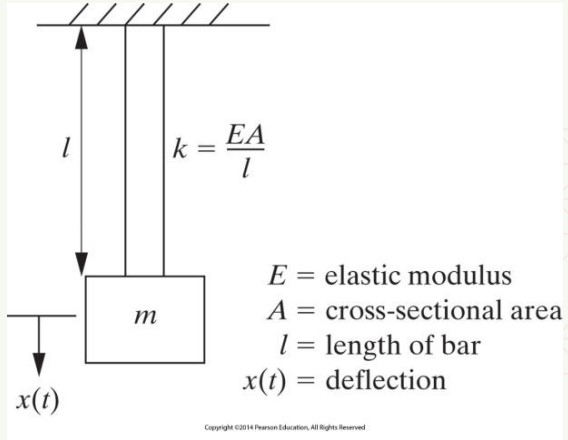
\includegraphics[width = 0.8\textwidth]{../img/diagram19.jpg}
    \caption{Longitudinal motion of a bar.}
\end{figure}
\subsection{Torsional rotation of a shaft}
\begin{figure}[H]
    \centering
    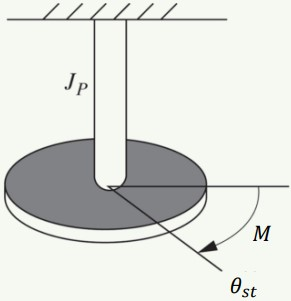
\includegraphics[width = 0.6\textwidth]{../img/diagram20.jpg}
    \caption{Torsional disc system.}
\end{figure}
\begin{align}
    M &= k_{eq} \theta_{st}\\
    k_{eq} &= \dfrac{GJ_p}{l}
\end{align}
\begin{itemize}
    \item $G$: Shear modulus of rigidity
    \item $J_p$: Polar second moment of area
    \item $l$: Length of the shaft
\end{itemize}
\end{document}